In the previous chapter, we have studied the conversion process with a classical example. Now we will study in detail a three-dimensional representation of cerebral veins. For now we are not interested in a study from a medical point of view, in fact our objective is to compare our technique with the commonly used ones. In Figure~\ref{fig:visus0} we can see the veins representation with our technique and the same model created with the marching cubes algorithm.

\begin{figure}[htb] %  figure placement: here, top, bottom
   \centering
   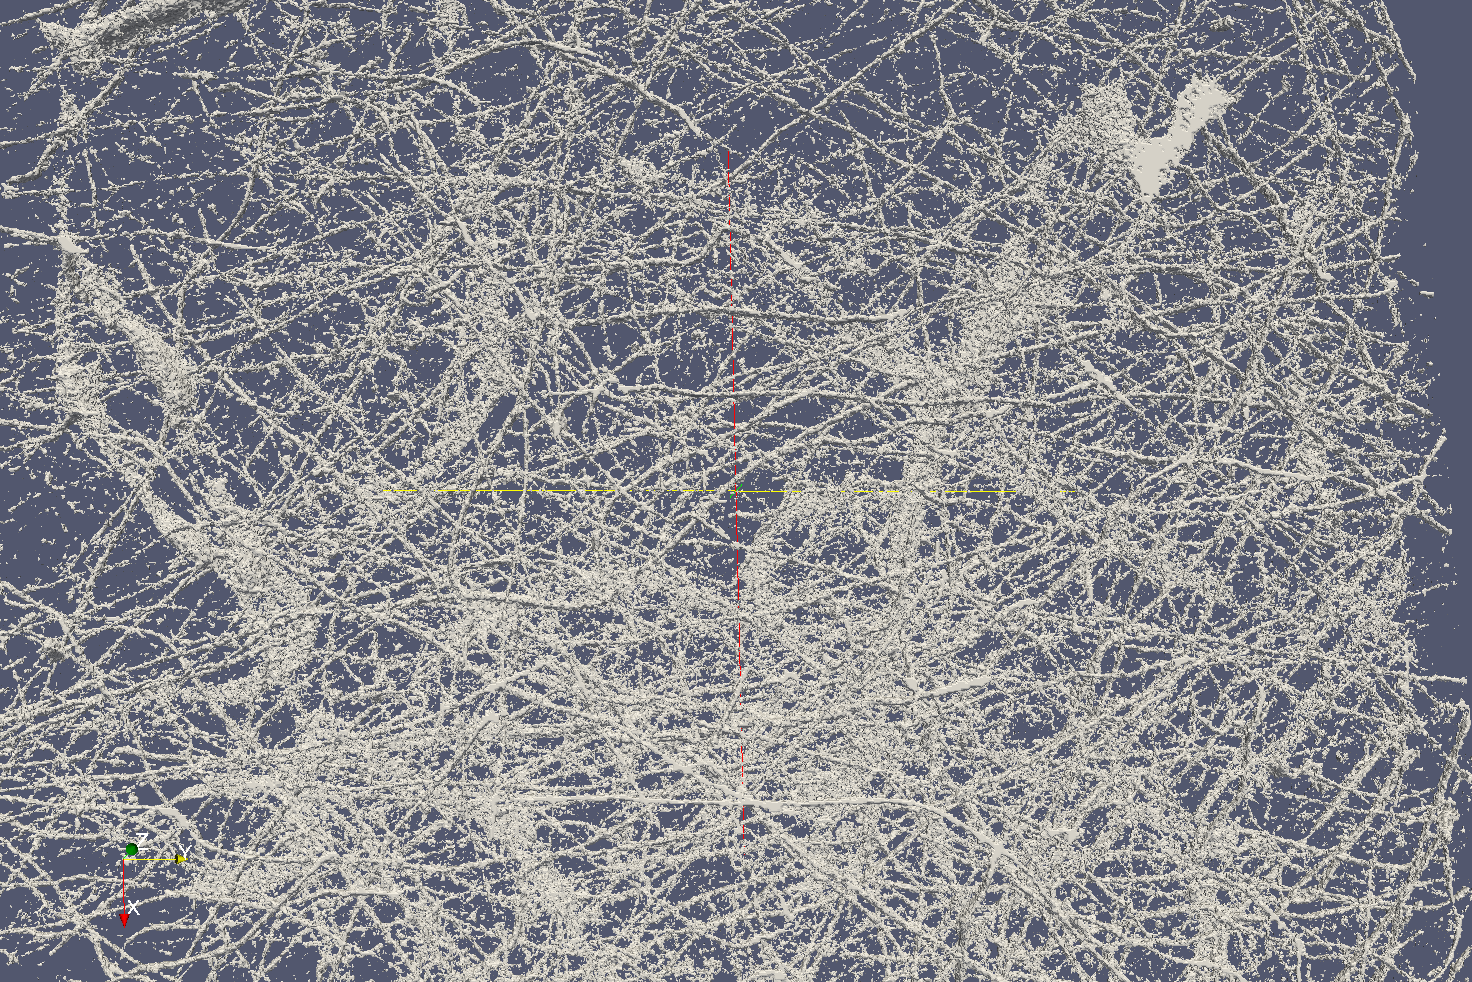
\includegraphics[width=0.49\linewidth]{images/LAR0.png}\hfill
   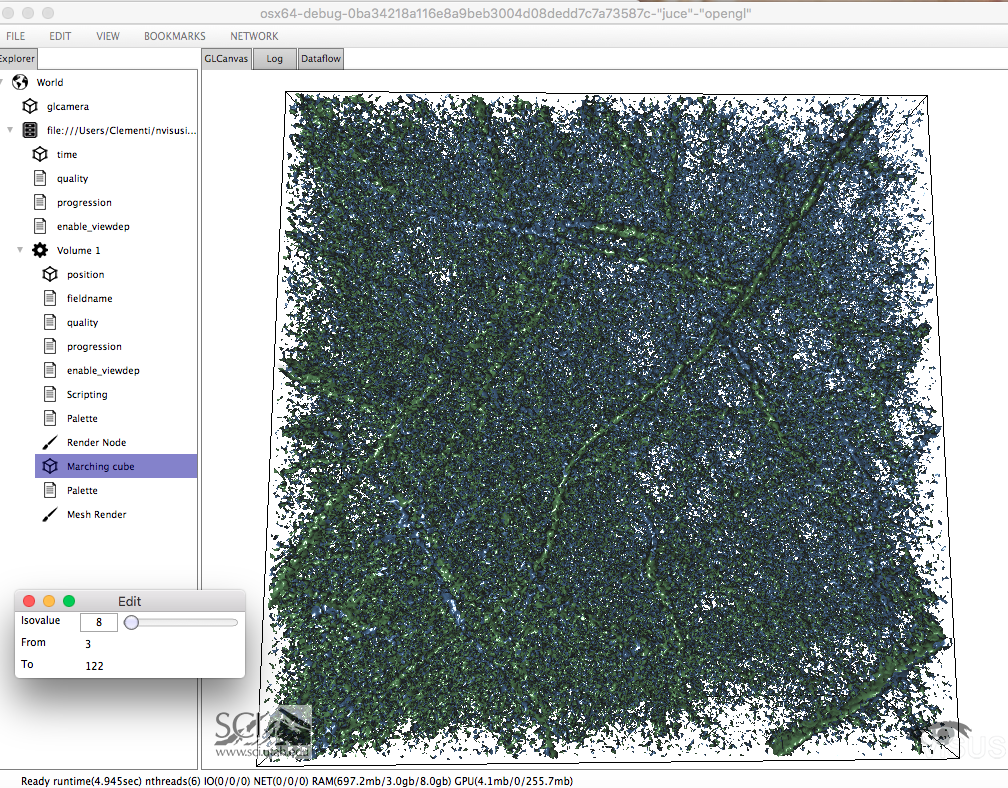
\includegraphics[width=0.49\linewidth]{images/visus0.png}
   \caption[Comparison between LAR and marching cubes]{Comparison between LAR and marching cubes. (a) A three-dimensional model of cerebral veins taken with our software. (b) The same model obtained from marching cubes and visualized in \textit{Visus} visualizer}
   \label{fig:visus0}
\end{figure}


From that figure, we can see that these two models seems similar when they are observed at a certain distance. However in Figure~\ref{fig:visus1} we can see that the reality is different.

\begin{figure}[htb] %  figure placement: here, top, bottom
   \centering
   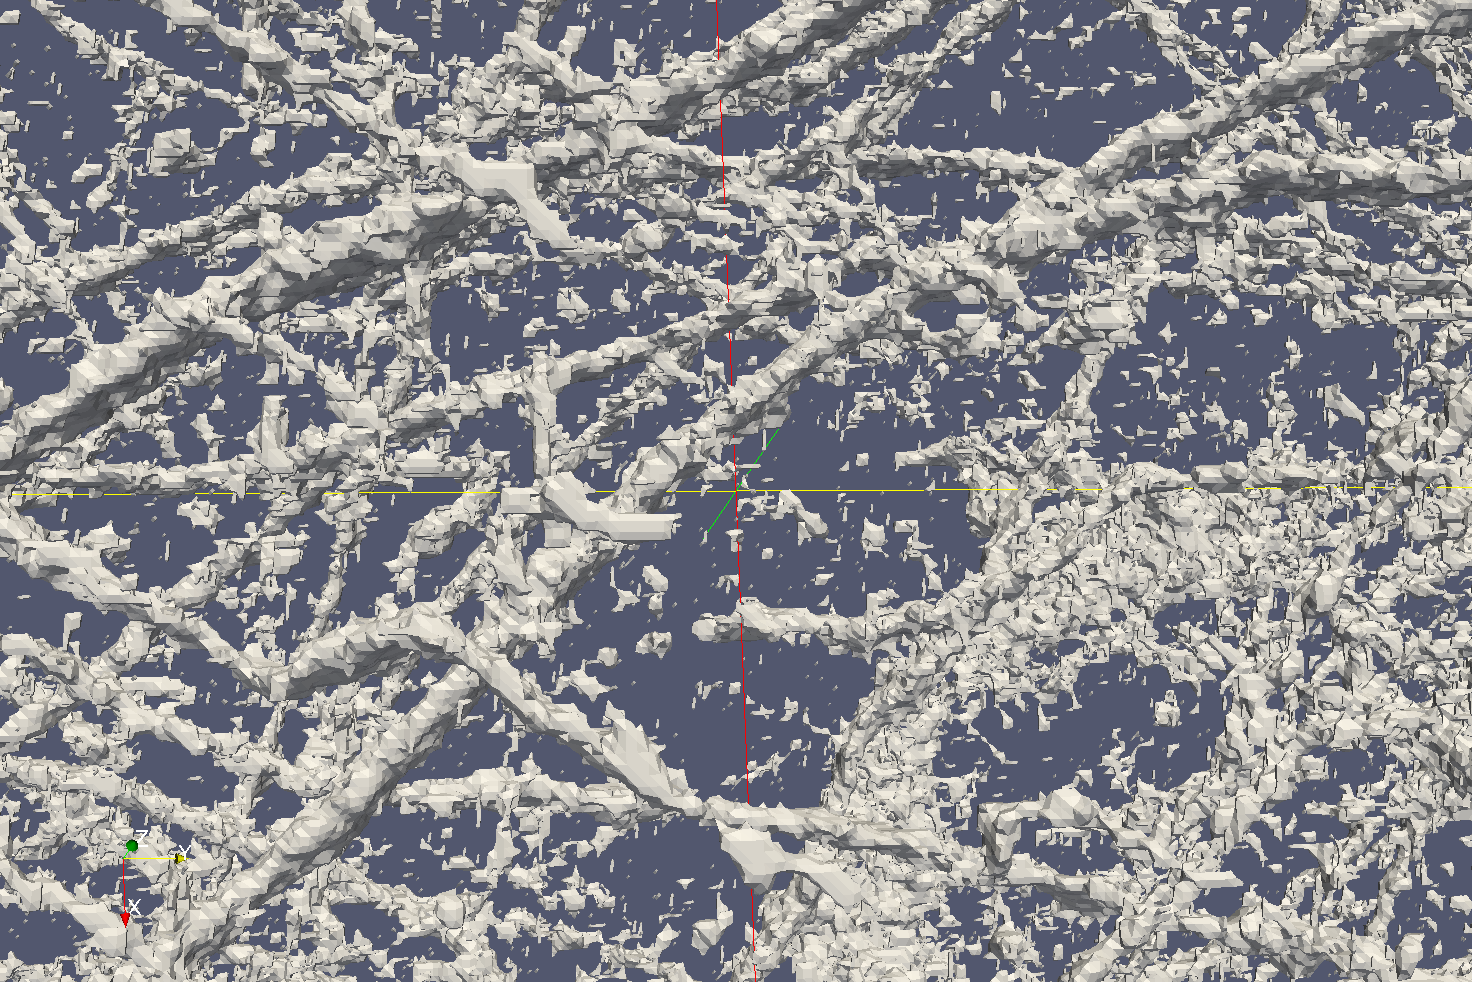
\includegraphics[width=0.33\linewidth]{images/LAR1.png}\hfill
   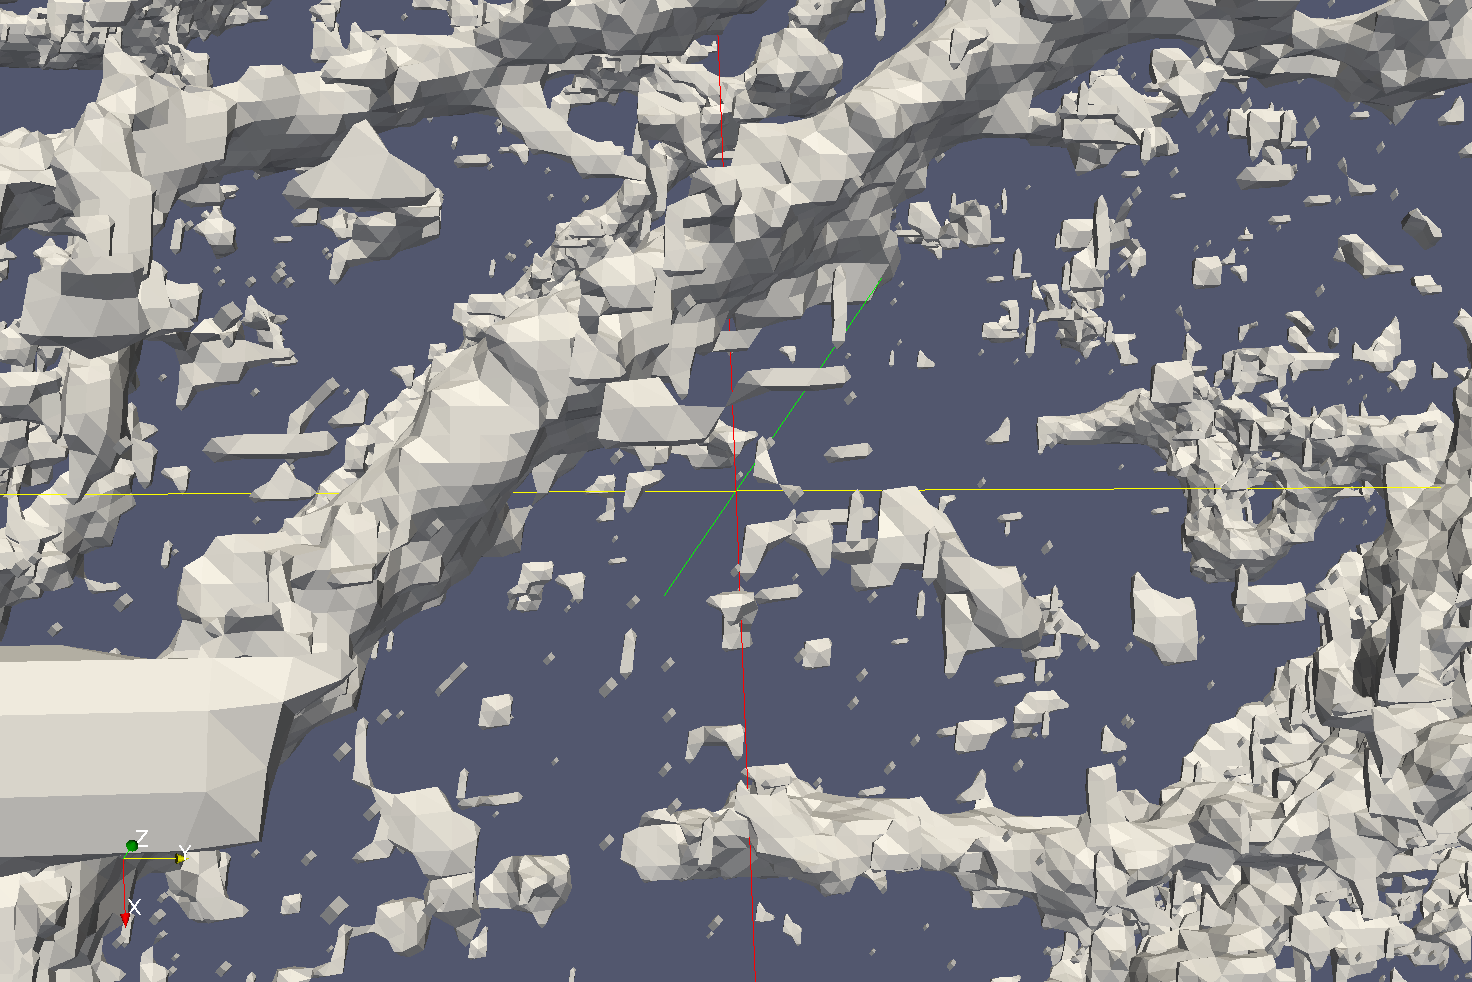
\includegraphics[width=0.33\linewidth]{images/LAR2.png}\hfill
   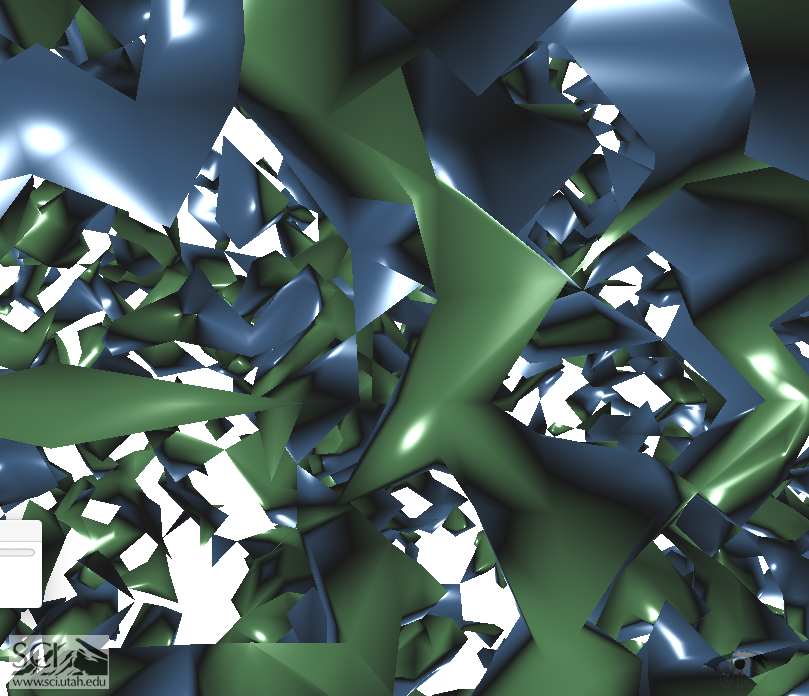
\includegraphics[width=0.33\linewidth]{images/visus1.png}
   \caption[Topological errors in marching cubes]{Topological errors in marching cubes. (a) and (b) Some images showing a zoomed portion of our three-dimensional model. (c) A zoomed view of the veins obtained from the marching cubes algorithm.}
   \label{fig:visus1}
\end{figure}

How we can see in that figure, while from a certain distance the models seems similar, a zoomed view shows all the errors caused by the marching cubes algorithm. In particular we can see that the topology of a single vein is completely lost. With LAR, instead, we do a \textit{topologically perfect} extraction saving the correct shape of the represented objects. In Figure~\ref{fig:larZoomed} we can see that every connected component (even noise) is closed.

\begin{figure}[htb] %  figure placement: here, top, bottom
   \centering
   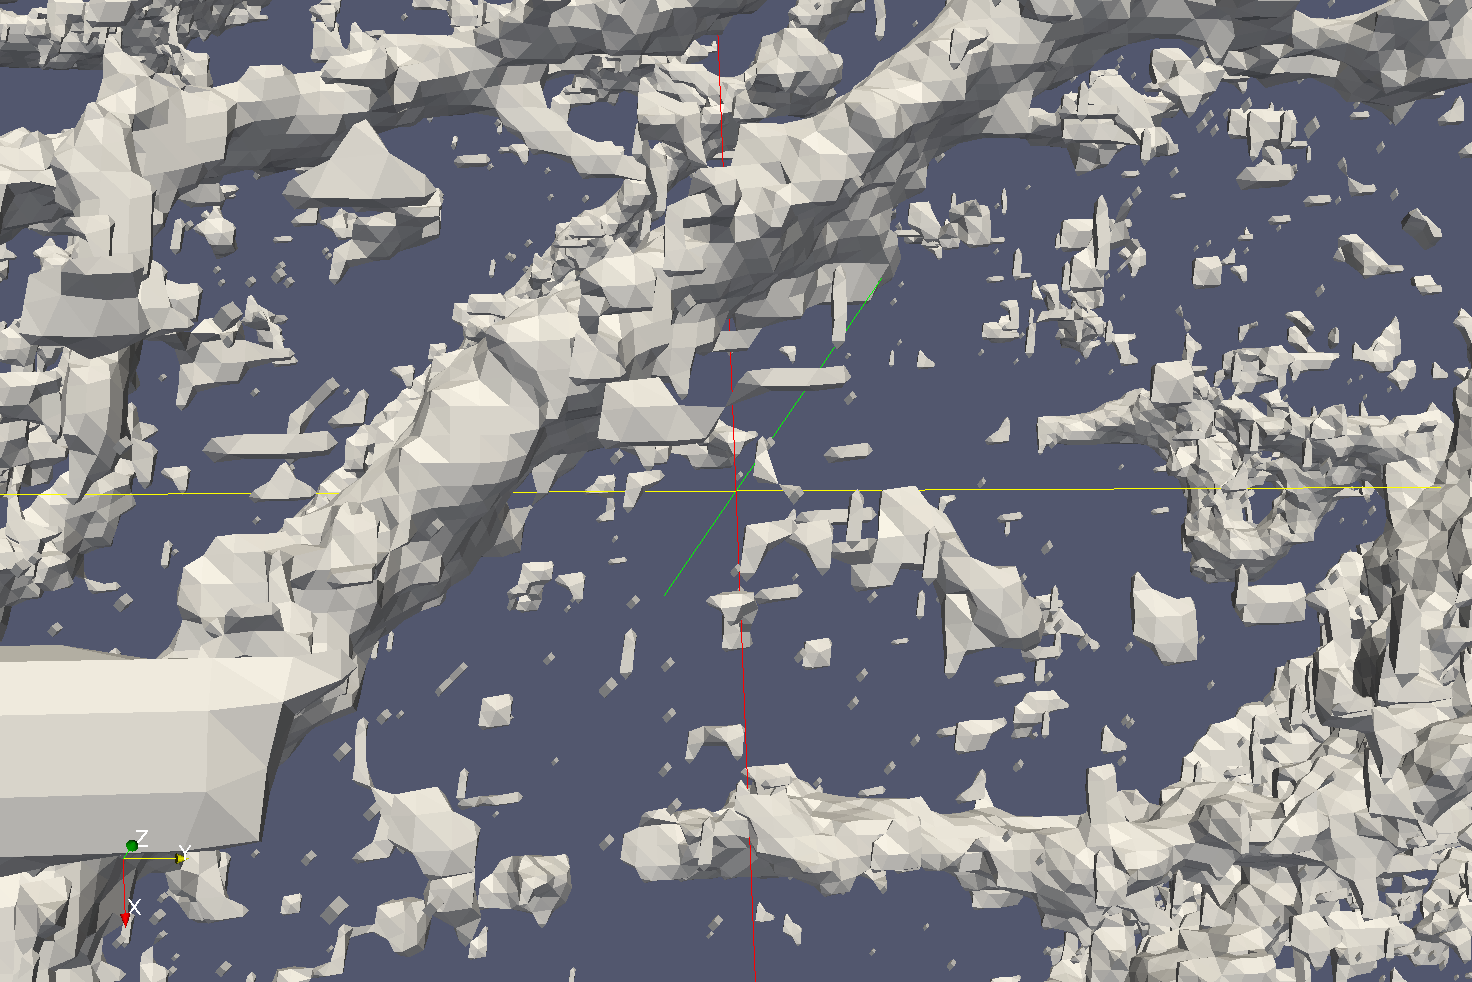
\includegraphics[width=0.50\linewidth]{images/LAR2.png}
   \caption[A close-up view of the LAR model]{A close-up view of the LAR model}
   \label{fig:larZoomed}
\end{figure}


\begin{figure}[htb] %  figure placement: here, top, bottom
   \centering
   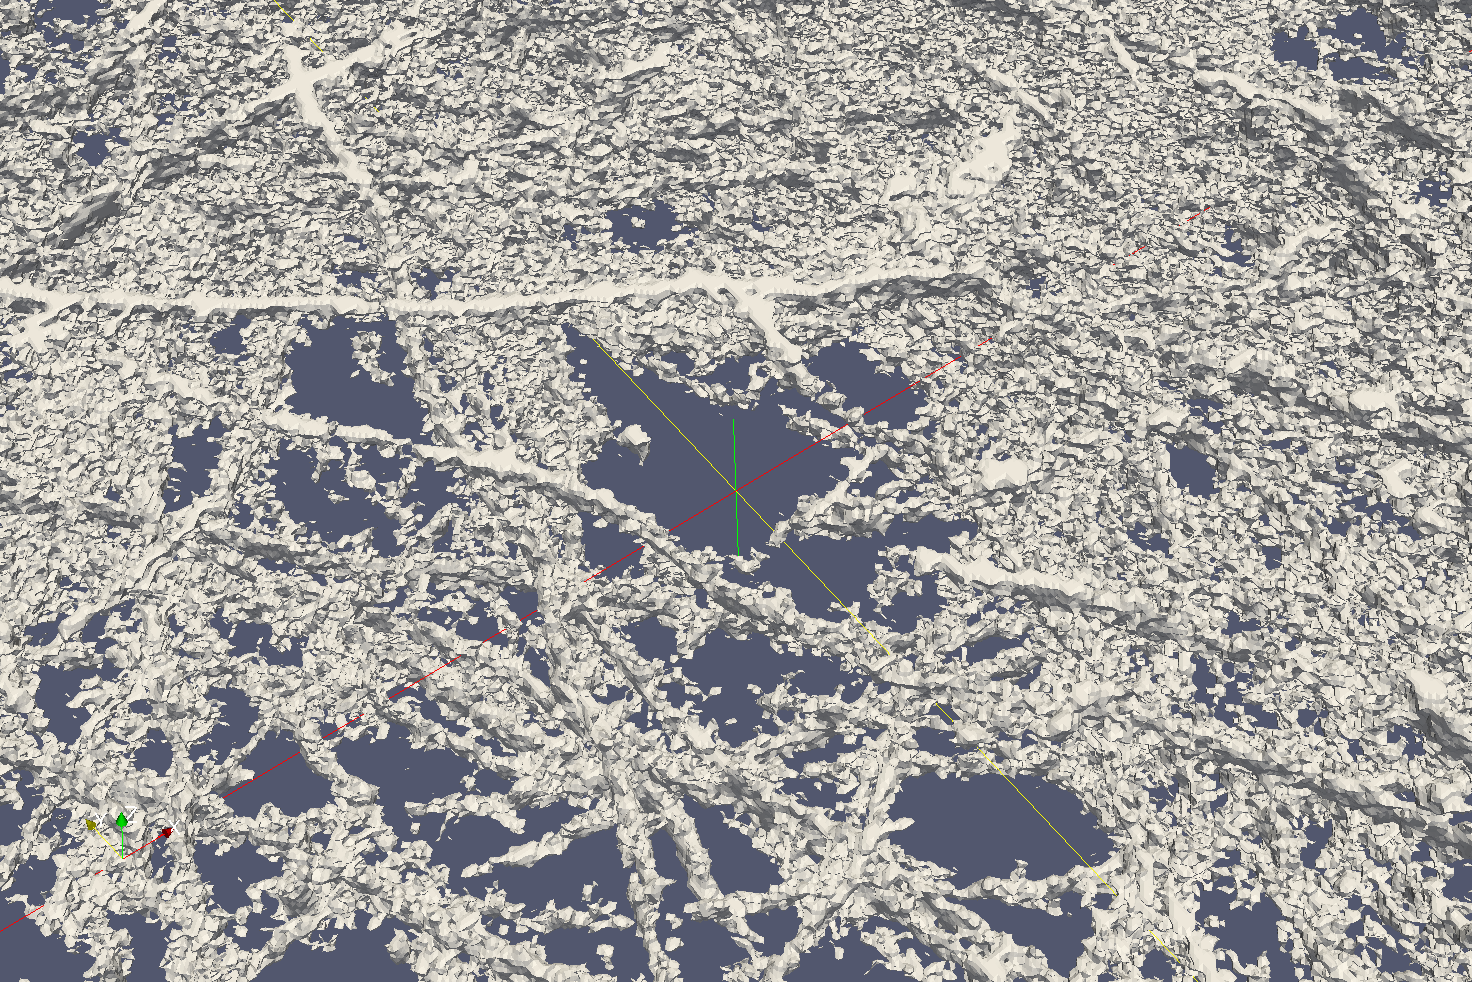
\includegraphics[width=0.49\linewidth]{images/NeuronsFil0.png}\hfill
   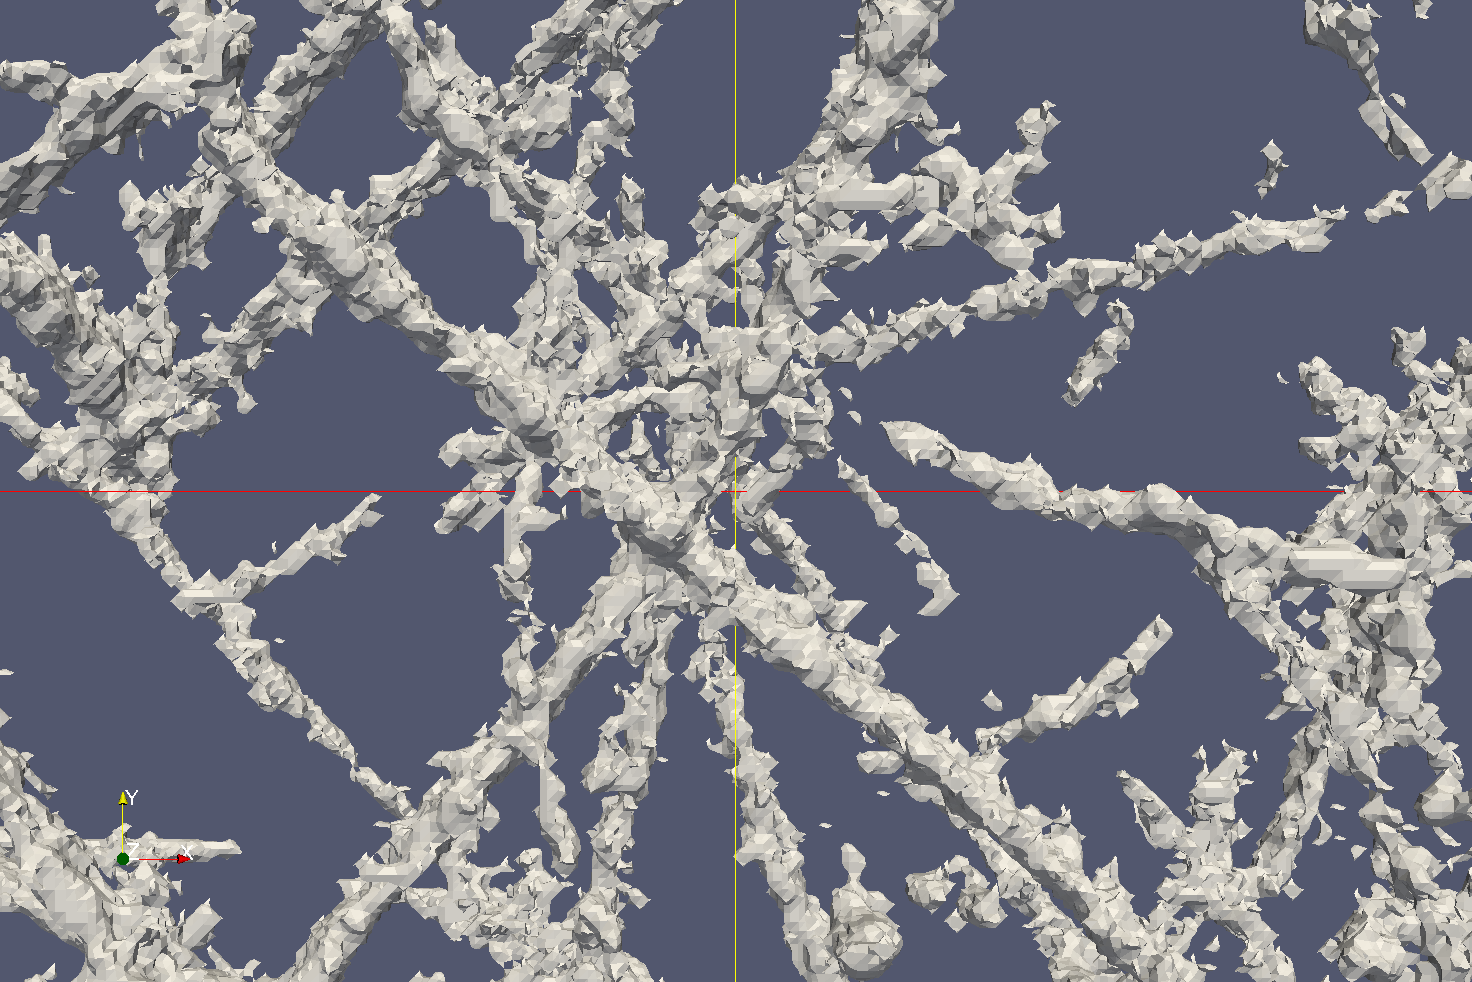
\includegraphics[width=0.49\linewidth]{images/NeuronsFil1.png}\newline
   
   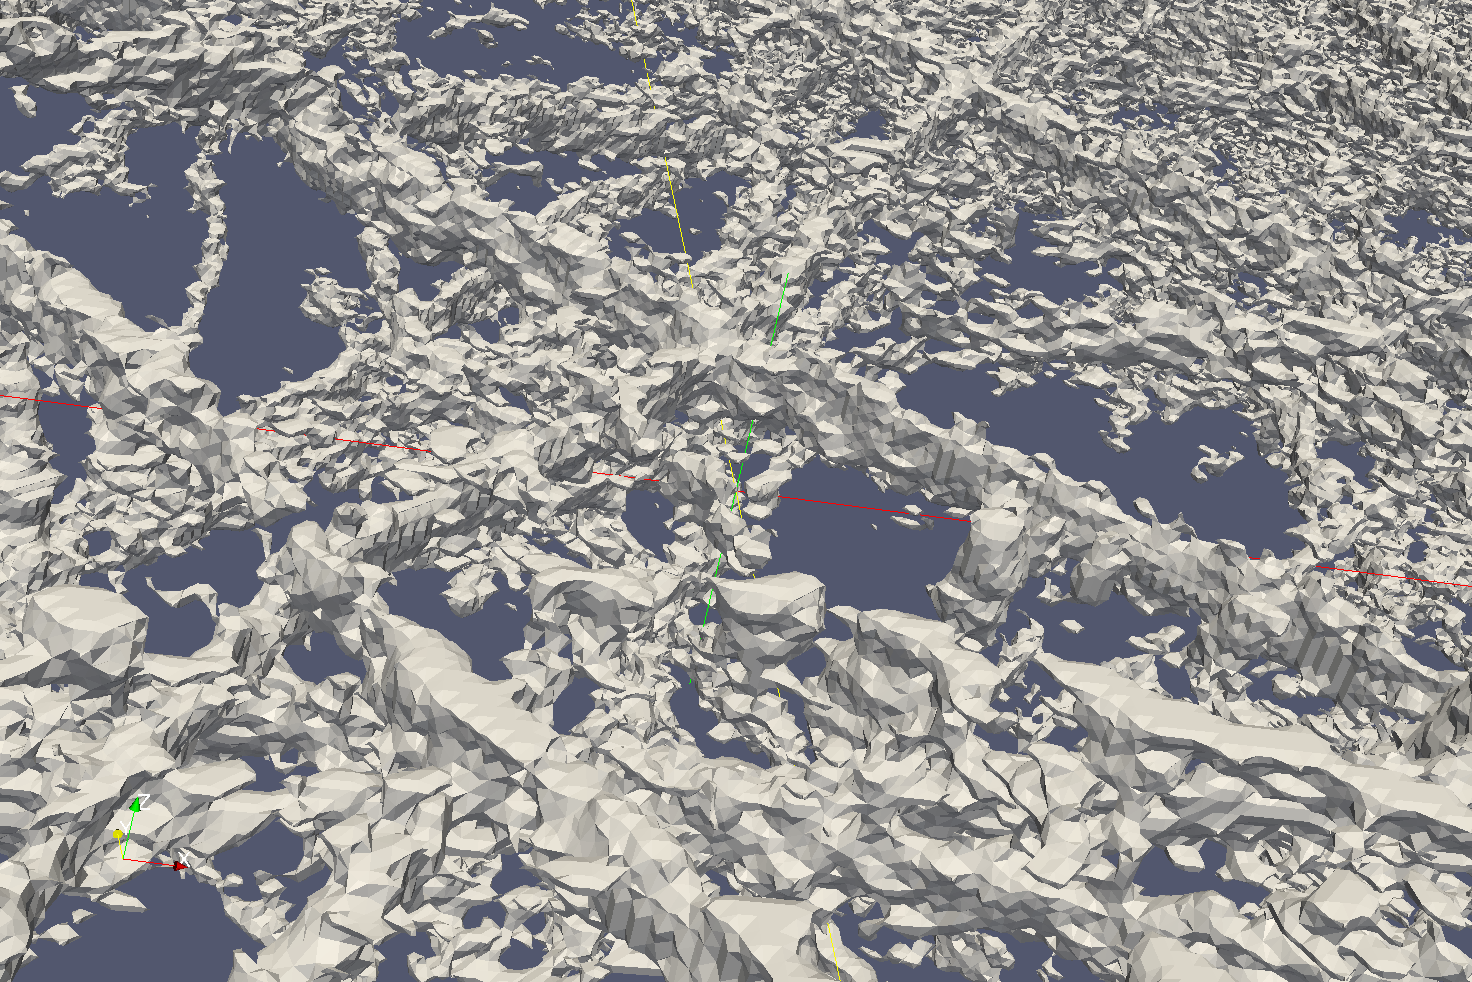
\includegraphics[width=0.49\linewidth]{images/NeuronsFil2.png}\hfill
   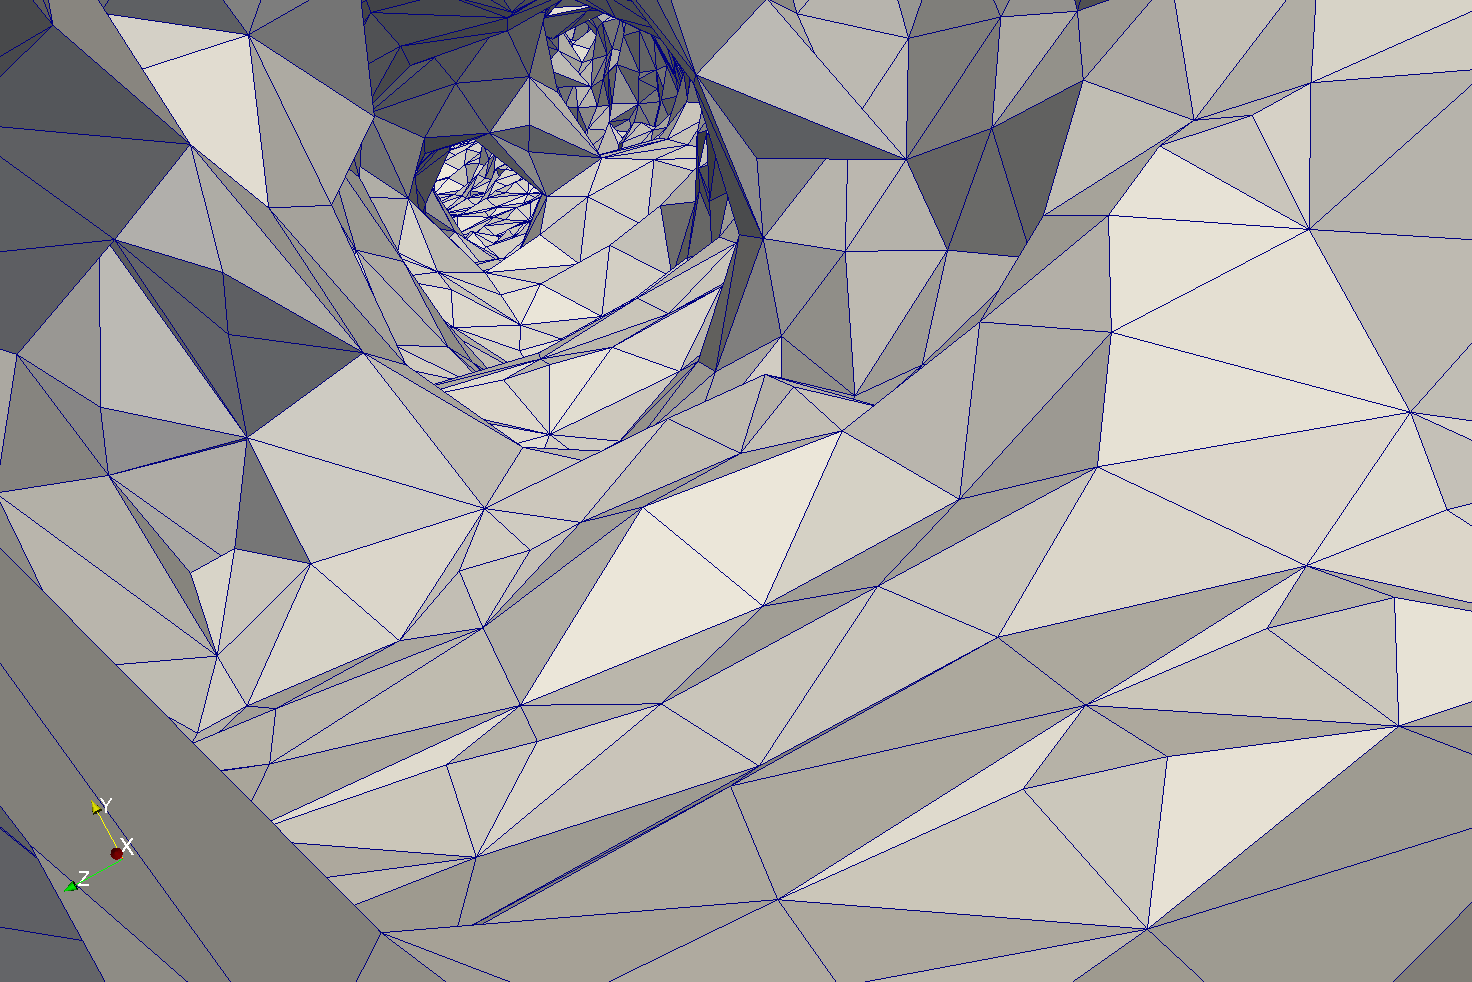
\includegraphics[width=0.49\linewidth]{images/NeuronsFil3.png}
   \caption[A detailed view of cerebral veins with LAR]{A detailed view of cerebral veins obtained with LAR. We can see all component are topologically correct (for example in (d) we can wee the interior of a vein)}
   \label{fig:larModelNeurons}
\end{figure}